%
\section{Statische Analyse}

\subsection{Gendarme}
Gendarme analysiert Programme und Bibliotheken, welche in den verschiedenen .NET Sprachen geschrieben wurden. Dafür benötigt Gendarme eine kompilierte Assembly, weil es nicht den C\# statisch analysiert, sondern ein daraus erzeugte Spracheformat: Das ECMA CIL.~\cite{ecma} Die CIL wird mit Hilfe von der Bibliothek Cecil analysiert.~\cite{cecil} Gendarme generiert auf Basis dieser Analyse Berichte. Sie können als HTML-Datei exportiert werden.

\paragraph{ECMA CIL}

\subsubsection{Fehler}

\subsubsection{Sicherheit}


\subsection{NDepend}
NDepend führt statischen Analysen von Projekten durch, erstellt dabei Softwarelandkarten, Codemetriken und überprüft ob Quelltextregel eingehalten werden.~\cite{ndepend} Auf der Dashboard genannten Übersicht erstellt NDepend eine Zusammenfassung aller Analysen.

\subsubsection{Quelltextregel}

\paragraph{Potentially dead Methods} In CSharpEssentials findet NDepend sechs mögliche Stellen, an denen Quelltext nicht ausgeführt wird. In Abbildung~\ref{fig:dead-methods} sieht man zwei der gefundenen Stellen. Bei allen handelt es sich um nicht aufgerufenen Konstruktoren. 

\begin{figure}[ht]
\centering
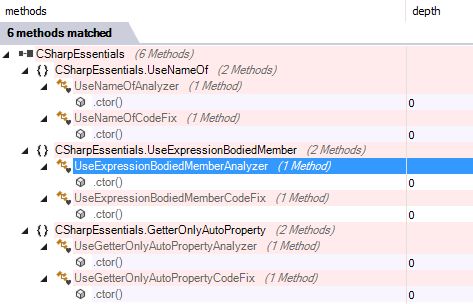
\includegraphics[width=0.7\textwidth]{images/dead-methods.png}
\caption[Potentially dead Methods]{\tabular[t]{@{}l@{}}Potentially dead Methods \\ Von NDepend gefundener wahrscheinlich nicht aufgerufener Quelltext\endtabular}
\label{fig:dead-methods}
\end{figure}

\subsection{Visual Studio Tools}
Visual Studio analysiert Code, erstellt dabei Quelltextmetriken und kann zum Beispiel Code-Clone identifizieren.

\subsubsection{Quelltextmetriken}

\subsubsection{Code-Clone}


\subsection{SourceMonitor}

\subsubsection{Kiviat-Chart}
